\section*{Sheet 6}
\subsection*{Exercise 1}
\begin{enumerate}[a)]
    \boldmath
    \item \textbf{For each $n \in N$ such that $n \geq 3$, give an easy example of a graph on n vertices where the smallest cardinality of a vertex cover is strictly greater than the maximum cardinality of a matching. Justify your answer.}
    \unboldmath
    \begin{figure}[h]
        \centering
        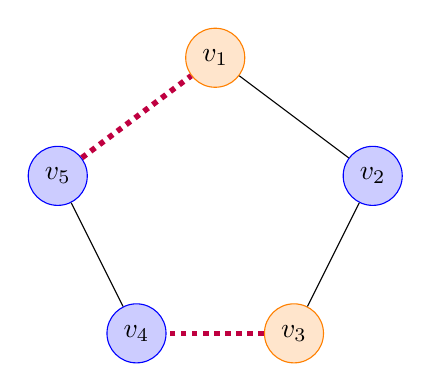
\begin{tikzpicture}
        \tikzset{
        dep/.style={circle,minimum size=0.75cm,fill=orange!20,draw=orange},
        vc/.style={circle, minimum
        size=0.75cm, fill=blue!20, draw=blue},
        c1/.style={-},
        c2/.style={dotted, purple, line width=2},
        }
        \node[dep] (n1) at (3,3) {$v_1$};
        \node[vc] (n2) at (5,1.5) {$v_2$};
        \node[dep] (n3) at (4, -0.5) {$v_3$}; 
        \node[vc] (n4) at (2, -0.5) {$v_4$};
        \node[vc] (n5) at (1, 1.5) {$v_5$}; 

        \draw[c1] (n1) edge node[above] {} (n2);
        \draw[c1] (n2) edge node[above] {} (n3);
        \draw[c2] (n3) edge node[above] {} (n4);
        \draw[c1] (n4) edge node[above] {} (n5);
        \draw[c2] (n5) edge node[above] {} (n1);
        \end{tikzpicture}
        \caption{The minimum vertex cover in \colorize{blue}{\textbf{blue}}, the maximum matching in \colorize {purple}{\textbf{purple}}}
    \end{figure}
    \\
    \linebreak
    \textbf{Justification}\\
    Any graph that is not isomorphic to a bipartite graph must contain a cycle of odd length. \\
    \linebreak
    If the graph $G$ contains a cycle of odd length, our vertex cover will just need $|U_G| = \ceil{\frac{n}{2}} + k$, where $U_G$ is the minimum vertex cover for the graph $G$, $n$ is the length of the cycle and $k$ is a constant value that accounts for the existence of other structures inside the graph that we are not caring for, at the moment.\\
    The above can be explained simply: since every vertex in the cycle has degree 2 then $\ceil{\frac{n}{2}} \cdot 2 > n$.\\
    \linebreak
    If we want to find the corresponding maximum matching we will have to build a walk like the one proposed below:
    \begin{center}
        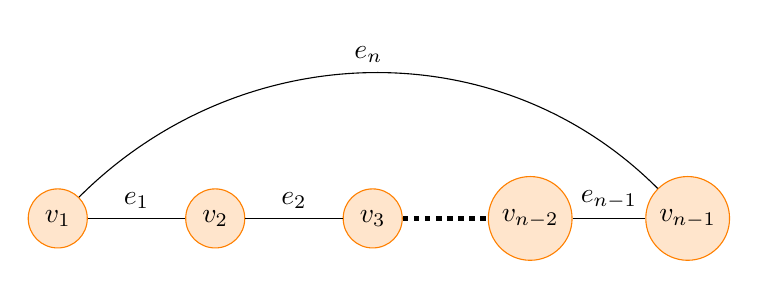
\begin{tikzpicture}
        \tikzset{
        dep/.style={circle,minimum size=0.75cm,fill=orange!20,draw=orange},
        vc/.style={circle, minimum
        size=0.75cm, fill=blue!20, draw=blue},
        c1/.style={-},
        c2/.style={dotted, purple, line width=2},
        c3/.style={dotted, black, line width=2},
        c4/.style={-, out=135, in=45}
        }
        \node[dep] (n1) at (-3,0) {$v_1$};
        \node[dep] (n2) at (-1,0) {$v_2$};
        \node[dep] (n3) at (1,0) {$v_3$}; 
        \node[dep] (n4) at (3,0) {$v_{n - 2}$};
        \node[dep] (n5) at (5,0) {$v_{n - 1}$}; 

        \draw[c1] (n1) edge node[above] {$e_1$} (n2);
        \draw[c1] (n2) edge node[above] {$e_2$} (n3);
        \draw[c3] (n3) edge node[above] {} (n4);
        \draw[c1] (n4) edge node[above] {$e_{n - 1}$} (n5);
        \draw[c4] (n5) edge node[above] {$e_n$} (n1);
        \end{tikzpicture}
    \end{center}
    We will consider the cycle $w = v_1e_1v_2 \dots v_{n - 2}e_{n - 1}v_{n - 1}e_nv_1$.\\
    \linebreak
    Since we are looking for the maximum matching $M$ we will look to add as many edges as possible to the set. Thus we will be alternating edges that are not in $M$ to edges that are in $M$. That translates into taking half of the edges in the cycle ($\frac{n}{2}$). Since, by hypothesis, we know that $n$ is odd then $n - 1$ is even. We can choose two different courses of action:
    \begin{itemize}
        \item $e_1 \in M$, then, by exclusion $e_n \notin M$
        \item $e_1 \notin M$, then, by exclusion $e_n \in M$
    \end{itemize}
    Overall, $|M| = \frac{n - 1}{2} = \floor{\frac{n}{2}}$, but
    \begin{equation}
        \floor{\frac{n}{2}} \leq \ceil{\frac{n}{2}} \label{eq:fundamental}
    \end{equation}
    In the specific case of the odd cycle we can actually say that the floor is strictly less than the ceiling $\implies$ that we will always have a maximum matching which is smaller than the minimum vertex cover.
    \boldmath
    \item \textbf{For each $m, n \in N$ such that $2 \leq m < n$, give an easy example of a graph G on n vertices and $A \subseteq V (G)$ of size m such that G has a matching of A but Hall’s condition does not hold. Justify your answer. (Recall that for a set S of vertices we defined $N(S) := \bigcup_{s\in S} N(s) \setminus S$)} \\
    \linebreak 
    \unboldmath
    As an example, let $m = 1$ and $n = 4$. This satisfies $2 \leq m < n$. In the graph below $A = \{v_4\}$. 
    \begin{figure}[h]
        \centering
        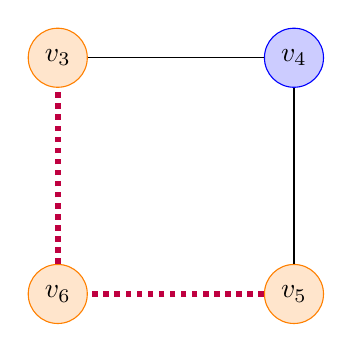
\begin{tikzpicture}
        \tikzset{
        dep/.style={circle,minimum size=0.75cm,fill=orange!20,draw=orange},
        vc/.style={circle, minimum
        size=0.75cm, fill=blue!20, draw=blue},
        c1/.style={-},
        c2/.style={dotted, purple, line width=2},
        c3/.style={dotted, black, line width=2},
        c4/.style={-, out=135, in=45}
        }
        \node[dep] (n3) at (3,1.5) {$v_3$}; 
        \node[vc] (n4) at (6,1.5) {$v_4$};
        \node[dep] (n5) at (6,-1.5) {$v_5$}; 
        \node[dep] (n6) at (3,-1.5) {$v_6$}; 
        
        \draw[c1] (n3) edge node[above] {} (n4);
        \draw[c1] (n4) edge node[above] {} (n5);
        \draw[c2] (n5) edge node[above] {} (n6);
        \draw[c2] (n6) edge node[above] {} (n3);
        \end{tikzpicture}
        \caption{vertices that belong to $A$ are in \colorize{blue}{\textbf{blue}}, the matching is in \colorize{purple}{\textbf{purple}}}
        \label{ex2}
    \end{figure}
    \\\linebreak
    \textbf{Justification}\\
    Let's suppose we have a graph $G$ that is not bipartite\footnote{We consider a non bipartite graph because Hall's condition is a necessary and sufficient condition for a bipartite graph to have an A-perfect matching}, we pick a generic $A \subseteq V(G)$ and we are looking for an A-perfect matching $M_A$, we also suppose Hall's condition doesn't hold, which means that $|N_G(A)| < |A|$.\\
    The only way for a matching to be formed without having $|N_G(A)| \geq |A|$ is that not all vertices have at least a neighbour outside of $A$.\\
    \linebreak
    If all of the vertices in $A$ have a neighbour that can be used to build $M_A$ but not all of the neighbours are $\notin A$ then we can define Kronecker's delta this way:
    \[
    \delta(v) =
    \begin{cases}
        0, & \text{if } v \in A \\
        1, & \text{if } v \notin A
    \end{cases}
    \]
    Now that we have defined the function we can conclude that, because of how we defined the neighbourhood relation over set of vertices:
    \begin{equation}
        N_G(A) = \bigcup_{v \in A} N_G(v) \setminus A = \sum_{v \in A} \delta(v) \leq |A|
    \end{equation}
    
    
\end{enumerate}
\textbf{(Remark: this shows that the “bipartite”condition in König’s and Hall’s theorems is necessary.)}
